\documentclass{ieeeaccess}
\usepackage{cite}
\usepackage{amsmath,amssymb,amsfonts}
\usepackage{graphicx}
\usepackage{textcomp}
\usepackage{bm}
\usepackage{url}
\makeatletter
\AtBeginDocument{\DeclareMathVersion{bold}
\SetSymbolFont{operators}{bold}{T1}{times}{b}{n}
\SetSymbolFont{NewLetters}{bold}{T1}{times}{b}{it}
\SetMathAlphabet{\mathrm}{bold}{T1}{times}{b}{n}
\SetMathAlphabet{\mathit}{bold}{T1}{times}{b}{it}
\SetMathAlphabet{\mathbf}{bold}{T1}{times}{b}{n}
\SetMathAlphabet{\mathtt}{bold}{OT1}{pcr}{b}{n}
\SetSymbolFont{symbols}{bold}{OMS}{cmsy}{b}{n}
\renewcommand\boldmath{\@nomath\boldmath\mathversion{bold}}}
\makeatother

\begin{document}
\history{Date of publication xxxx 00, 0000, date of current version xxxx 00, 0000.}
\doi{10.1109/ACCESS.2024.0429000}

\title{Why Quantum Reservoirs Do Not Improve Intraday Commodity Volatility Forecasts: A Memory Mismatch Confirmed in a Publicly Pre-Registered Held-Out Test}

\author{\uppercase{Sandanayakage Janindu Indira Sandanayaka}\authorrefmark{1},
\uppercase{Maninda Edirisooriya}\authorrefmark{1}, AND \uppercase{Achala Aponso}\authorrefmark{1}}

\address[1]{Informatics Institute of Technology, Colombo, Sri Lanka, in collaboration with the University of Westminster, London, U.K. (e-mail: janindu.20232270@iit.ac.lk)}

\tfootnote{This work did not receive any specific funding.}

\markboth
{S. J. I. Sandanayaka \headeretal: Quantum Reservoirs and Intraday Commodity Volatility}
{S. J. I. Sandanayaka \headeretal: Quantum Reservoirs and Intraday Commodity Volatility}

\corresp{Corresponding author: S. J. I. Sandanayaka (e-mail: janindu.20232270@iit.ac.lk).}

\begin{abstract}
Quantum reservoir computers have been reported to beat classical volatility forecasts, but it is unclear when such an advantage is possible. We compare two quantum reservoirs of a published design with tuned classical reservoirs, recurrent neural networks, the heterogeneous autoregressive model and a 200-lag linear model on the realized volatility of copper futures sampled every 5, 15 and 60 minutes from 2013 to 2026. No quantum reservoir improves on the strong classical models by more than 3\%, and at 15 and 60 minutes they are 1.5\% to 2.8\% worse than the linear model. The reason is a memory mismatch: the reservoirs keep 90\% of their linear memory within 5 to 8 steps, while the signal left in copper volatility after the autoregressive benchmark lies 50 to 200 steps back. On synthetic data, a quantum reservoir gains only when it is the circuit that generated the data. We then publicly registered three predictions before obtaining the minute-level gold and silver data, and tested them once. All three held: no quantum edge in 24 comparisons, the remaining signal beyond the reservoirs' memory in all six market and frequency cells, and no information beyond a classical reservoir of the same memory in all six. Finally, we show that ordinary evaluation choices, made after seeing test results, can turn the copper result into an apparent quantum advantage of nearly 20\%, whereas choosing the same options at random does not. For these reservoirs and data, matching memory to the data matters more than quantum design.
\end{abstract}

\begin{keywords}
Commodity futures, forecast evaluation, pre-registration, quantum machine learning, quantum reservoir computing, realized volatility, reservoir memory.
\end{keywords}

\titlepgskip=-21pt

\maketitle

\section{Introduction}
\label{sec:introduction}
\PARstart{Q}{uantum} reservoir computing (QRC) drives a fixed quantum system with the input and trains only a linear readout of measured observables. Because only the readout is trained, QRC is attractive for near-term quantum hardware, and recent studies report that it forecasts financial volatility better than classical models \cite{li2026}. Other work finds no such advantage once classical baselines are tuned with equal care \cite{pandey2026,maheshwari2026b}, and benchmarks of quantum machine learning (QML) on time series find that quantum models rarely beat classical models of comparable size \cite{fellner2026}.

Intraday volatility forecasts are used for risk limits, margin requirements, option pricing and the execution of large orders, and metal futures are among the most actively traded commodity contracts. Volatility is persistent: its autocorrelation decays slowly over many days, which is why simple models that average past realized variance over several horizons are hard to beat \cite{andersen2003,corsi2009}. Any new model, quantum or classical, must therefore be compared with such benchmarks and must be able to use information from far in the past.

Two questions remain open. First, when could a quantum reservoir help? A reservoir can only use the parts of the past it remembers, so its memory must reach the lags at which the data still carry information \cite{dambre2012}. We did not find a study that compares the memory of quantum reservoirs with the lag structure of real financial data. Second, most comparisons are made on data the authors have already examined, so their conclusions are exposed to choices made after seeing results \cite{bowles2024,white2000}. A test on data that the authors have not seen, with predictions fixed in public beforehand, removes that exposure.

We study intraday realized volatility of copper, gold and silver futures and ask four questions.
\begin{enumerate}
\item Under a sound protocol, do two quantum reservoirs of a published design \cite{domingo2026} beat strong classical models on copper?
\item If not, why not?
\item Do the copper findings hold on assets whose minute-level data the authors had never loaded, under a public pre-registration?
\item How could ordinary evaluation choices nevertheless produce an apparent quantum advantage?
\end{enumerate}

Our contributions are as follows.
\begin{itemize}
\item A three-tier comparison on copper at 5-, 15- and 60-minute sampling from 2013 to 2026, including tuned classical reservoirs, classical models that copy the algebraic form of the quantum update, recurrent networks and a 200-lag linear benchmark (Section~\ref{sec:res-copper}).
\item A memory mechanism: the reservoirs' memory is far shorter than the lags at which copper's remaining signal sits. A synthetic positive control shows when a quantum reservoir can gain (Sections~\ref{sec:res-mech} and~\ref{sec:res-map}).
\item A publicly pre-registered, held-out test on gold and silver in which three predictions derived from copper were all confirmed (Section~\ref{sec:res-heldout}).
\item A measurement of how much apparent quantum advantage evaluation choices made after seeing test results can create, and how often such choices appear in published QML forecasting papers (Section~\ref{sec:res-choices}).
\end{itemize}
A companion study audits a published QRC volatility claim on its authors' own data \cite{companion}; this paper uses none of its data or results.

\section{Related Work}
\label{sec:related}

\subsection{Quantum Reservoirs and Their Classical Counterparts}
Domingo \emph{et al.} designed gate-based and Ising quantum reservoirs for market forecasting \cite{domingo2026}. Quantum reservoirs of finite dimension belong to the class of state-affine systems studied in classical reservoir computing \cite{martinezpena2023}, and their outputs are truncated Fourier series of the inputs \cite{schutte2025}. The information processing capacity of Dambre \emph{et al.} quantifies the memory and nonlinearity a reservoir offers \cite{dambre2012}. Nguyen and Soh reported a quantum reservoir that beats a tuned echo state network on a chaotic benchmark \cite{nguyen2026}.

\subsection{Memory in Reservoir Computing}
A reservoir forecasts well only if its state still carries the parts of the input history that matter for the target. Jaeger introduced the short-term memory capacity, the summed ability of a linear readout to reproduce past inputs \cite{jaeger2004}, and Dambre \emph{et al.} showed that total capacity is bounded by the number of independent state variables, so memory and nonlinearity compete for the same resource \cite{dambre2012}. Small quantum reservoirs have few measured observables and lose information each time a qubit is reset, which suggests short memory. Whether that memory is long enough for a given forecasting task is an empirical question that, to our knowledge, has not been asked for financial data.

\subsection{Quantum Models for Financial Forecasting}
Li \emph{et al.} reported that a quantum reservoir improves monthly volatility forecasts \cite{li2026}. Maheshwari \emph{et al.} reported a modest edge of quantum recurrent models \cite{maheshwari2026a}, which disappeared in their later study with more seeds, matched controls and naive baselines \cite{maheshwari2026b}. Shen found that a quantum kernel for stock returns looks dominant only on a universe screened with full-sample information \cite{shen2026}.

\subsection{Evaluation Practice}
Bowles \emph{et al.} showed that careful benchmarking removes most claimed QML advantages in classification \cite{bowles2024}; Islam showed that evaluation choices can reverse conclusions with the models fixed \cite{islam2026}; and Pandey showed that reported QRC gains vanish against classical models with the same size and tuning budget \cite{pandey2026}. Seed variance, leakage and weak baselines distort machine-learning comparisons more generally \cite{bouthillier2021,kapoor2023,arp2022}, and searching over many specifications inflates the best result \cite{white2000,hansen2005,harvey2016,bailey2014,simonsohn2020}. Table~\ref{tab:closest} summarizes how this work differs from the closest studies. Pre-registration and specification curves were proposed to make such searches visible \cite{simonsohn2020}; in finance, Harvey \emph{et al.} argued that the threshold for a new discovery must rise with the number of tests tried \cite{harvey2016}.

\begin{table}[t]
\caption{What the Closest Studies Examine}
\label{tab:closest}
\centering
\begin{tabular}{p{1.55cm}p{1.45cm}ccc}
\hline
Study & Data & Memory vs. data lags & Same-memory classical twin & Public held-out test \\
\hline
Li \emph{et al.} \cite{li2026} & monthly volatility & no & no & no \\
Pandey \cite{pandey2026} & synthetic & no & size-matched & no \\
Shen \cite{shen2026} & stock returns & no & no & no \\
Maheshwari \emph{et al.} \cite{maheshwari2026b} & financial series & no & matched controls & no \\
This work & intraday volatility & yes & yes & yes \\
\hline
\end{tabular}
\end{table}

\section{Data}
\label{sec:data}
We use one-minute bars of the most-traded copper, gold and silver futures traded on COMEX, the commodity exchange of CME Group (Databento continuous series HG.v.0, GC.v.0 and SI.v.0, June 2010 to 16 October 2026). For each bin of 5, 15 or 60 minutes, the target is the logarithm of realized variance, the sum of squared log differences of consecutive one-minute closes within the bin and the same contract \cite{andersen2003}; a bin is used if it holds at least 2, 3 or 5 one-minute bars. Each forecasting block covers one calendar year $Y$: models are trained on years $Y-4$ to $Y-2$, tuned on $Y-1$, and tested on $Y$, with a 24-hour gap between the parts. Rolling test years are 2013 to 2025 and the period from January to mid-October 2026 is held out. For copper the rolling test sets have 673,104, 283,953 and 67,567 rows at 5, 15 and 60 minutes. The Databento data are licensed and cannot be shared. Table~\ref{tab:samples} gives the number of test bins.

\begin{table}[t]
\caption{Number of Test Bins}
\label{tab:samples}
\centering
\begin{tabular}{llrrr}
\hline
Asset & Test period & 5 min & 15 min & 60 min \\
\hline
Copper & 2013--2025 & 673,104 & 283,953 & 67,567 \\
Copper & 2026 & 49,865 & 17,908 & 4,151 \\
Gold & 2026 & 55,027 & 18,151 & 4,141 \\
Silver & 2026 & 53,150 & 17,979 & 4,145 \\
\hline
\multicolumn{5}{p{7.6cm}}{\footnotesize 2026: January to 16 October. The gold and silver purchase held 5,674,801 and 5,244,708 one-minute bars.}\\
\end{tabular}
\end{table}

The authors had not loaded minute-level gold or silver data from any source before the public registration of Section~\ref{sec:protocol}, and no model had been fitted to 5- or 15-minute gold or silver data. They had seen gold and silver at daily frequency (gold test years 2013 to 2017 and 2020 to 2025; silver 2020 to 2025) and as hourly bars from another source (May 2024 to October 2026).

\section{Models}
\label{sec:models}
All models forecast the next bin's log realized variance (Table~\ref{tab:models}).

\textit{Econometric tier.} The heterogeneous autoregressive (HAR) model \cite{corsi2009} regresses $x_{t+1}$, the log realized variance of bin $t+1$, on
\begin{equation}
x_{t+1}=\boldsymbol{\beta}^{\top}\mathbf{z}_t+\textstyle\sum_{h}\gamma_h D_{h,t+1}+\varepsilon_{t+1},
\label{eq:har}
\end{equation}
where $\mathbf{z}_t$ holds a constant, $x_t$, and the means of $x$ over the last 10 bins, one day and five days, and $D_h$ are hour-of-day dummies. LIN200 adds a ridge regression on the last 200 values of $x$, fitted to the HAR residual with the penalty chosen on the tuning year.

\textit{Classical machine learning.} Echo state networks \cite{jaeger2004} with 28 units and input scale 0.5 read the same single series as the quantum reservoirs; ESN28u\_t is tuned over spectral radius $\{0.6,0.9,1.2\}\times$ leak rate $\{0.1,0.2,0.5,1.0\}$. Two classical twins copy the algebraic form of the quantum update: a state-affine system whose update is linear in the state with coefficients $1-u$, $u$ and $\sqrt{u(1-u)}$ (SAS28\_t), and an echo state network fed the same two input functions (ESNq\_t). The state-affine twins are tuned over gain $\{0.3,0.5,0.65\}\times$ leak rate $\{0.1,0.2,0.5,1.0\}$, and ESNb\_t and SASb\_t use a 256-number state read through 28 random projections. Reservoir settings are chosen by validation error averaged over two tuning seeds. Long short-term memory (LSTM) \cite{hochreiter1997} and gated recurrent unit (GRU) \cite{cho2014} networks read five channels (return, log realized variance, log volume, and the sine and cosine of the hour) over the last 10 bins; LSTM1 and GRU1 read the single series only. Networks are tuned over hidden size $\{8,16,32\}\times$ learning rate $\{3\times10^{-4},10^{-3},3\times10^{-3},10^{-2}\}$ on one tuning seed and trained with Adam, batch size 512 and at most 30 epochs with early stopping after 4 epochs without validation improvement.

\textit{Quantum reservoirs.} DOM is the gate-based reservoir of Domingo \emph{et al.} \cite{domingo2026}: seven qubits, one of which is reset each step to $\sqrt{1-u}\,|0\rangle+\sqrt{u}\,|1\rangle$, where $u$ is the input scaled to $[0,1]$ on training data; a fixed random circuit of 150 gates from $\{\mathrm{CNOT},\mathrm{H},\mathrm{T}\}$ acts each step, and the expectations of $X$ and $Z$ on every qubit after half and all of the circuit give 28 features. ISING replaces the circuit with evolution under a transverse-field Ising Hamiltonian with random couplings. Both are simulated exactly with density matrices, without shot noise.

\textit{Readout, seeds and computation.} All reservoirs use the same ridge readout on standardized features, fitted to the HAR residual, with the penalty chosen on the tuning year from $\{10^{-2},10^{-1},\dots,10^{3}\}$; LIN200 uses the same grid. Each stochastic model is run with 10 seeds and the forecasts are averaged. Computations used Python 3.12 with NumPy 2.5, SciPy 1.18 and PyTorch on an Intel Core Ultra 9 185H laptop CPU.

\begin{table}[t]
\caption{Models Compared}
\label{tab:models}
\centering
\begin{tabular}{lll}
\hline
Tier & Model & Input \\
\hline
Econometric & HAR, LIN200 & one series \\
Classical reservoir & ESN28u\_t & one series \\
Classical twin & ESNq\_t, SAS28\_t, ESNb\_t, SASb\_t & one series \\
Neural network & LSTM1, GRU1 & one series \\
Neural network & LSTM, GRU & five channels \\
Quantum reservoir & DOM, ISING & one series \\
\hline
\end{tabular}
\end{table}

\section{Evaluation Protocol}
\label{sec:protocol}
\textit{Copper.} Before each copper analysis, its plan (models, rows, statistics and decision rules) was written to a file whose SHA-256 hash, with the hashes of the code, was stored locally. These plans were made in sequence, each after earlier results had been seen, and the hashes have no third-party time stamp; the copper analyses are therefore confirmatory only within each step. Table~\ref{tab:regs} lists the steps in order.

\begin{table}[t]
\caption{Order of the Registered Analyses}
\label{tab:regs}
\centering
\begin{tabular}{p{0.35cm}p{3.3cm}p{3.5cm}}
\hline
Step & Analysis & Known when registered \\
\hline
1 & Copper comparisons with classical reservoirs, twins and networks (four rounds) & results of each earlier round \\
2 & 200-lag linear benchmark & all copper comparisons \\
3 & Memory functions and lag probe & all copper comparisons \\
4 & Synthetic positive control (two runs) & copper results; first run's error \\
5 & Evaluation choices on saved forecasts (three registrations) & all copper results \\
6 & Gold and silver held-out test (public, OSF) & copper results; no minute-level gold or silver data \\
\hline
\end{tabular}
\end{table}

\textit{Gold and silver.} The held-out test was registered publicly on the Open Science Framework (OSF) Registries \cite{osf2026} before the minute-level gold and silver data were bought. Its predictions were derived from the copper results and theory only, its models, code and statistics are copies of the copper ones with only the data paths changed, and its scripts are fixed by SHA-256 hashes listed in the registration. All deviations are listed in Appendix~\ref{app:deviations}.

\textit{Statistics.} For models $A$ and $B$ we report the ratio of total squared errors of log realized variance,
\begin{equation}
R_{A/B}=\frac{\sum_t (x_t-\hat{x}^A_t)^2}{\sum_t (x_t-\hat{x}^B_t)^2},
\label{eq:ratio}
\end{equation}
which is below 1 when $A$ is better, with a 95\% interval from the Newey-West variance \cite{newey1987} of the loss difference using one day of lags. $p$-values are Holm-adjusted \cite{holm1979} within each registered family. Each comparison falls into one of four categories with a $\pm3\%$ band: \emph{meaningful edge} (adjusted $p<0.05$ and the whole interval below 0.97), \emph{detectable, below band} (interval below 1), \emph{detectably worse} (interval above 1), or \emph{no detectable difference}.

\section{Mechanism and Positive-Control Methods}
\label{sec:methods-mech}
\textit{Memory.} On independent uniform inputs $u_t$ we fit a ridge readout to reproduce $v_{t-k}=2u_{t-k}-1$ and score it by $R^2$ on held-out steps; the memory function is $\max(0,R^2)$ for $k=0,\dots,400$ \cite{dambre2012}, and we report the lag below which 90\% of the total memory lies. On each asset we measure where the signal left by HAR sits: a ridge regression of the HAR residual on the last $K$ values, fitted on 2013 to 2022 and tested on 2023 to 2025; $K^*$ is the smallest $K$ that reaches 90\% of the best out-of-sample $R^2$.

\textit{Positive control.} Synthetic inputs follow a linear process with long or short memory, and the target adds a purely nonlinear signal produced by a \emph{teacher}: a DOM circuit, an Ising reservoir, an echo state network, a state-affine system, or a product of two or three lagged inputs. The signal's share of the residual variance is 2\%, 5\%, 15\% or 30\%, plus a null. There are 50 cells with 10 independent datasets each. The quantum students use circuits different from the teacher's, and the test is valid only if the teacher's own circuit beats the best classical student in a quantum-generated cell. A first run of this map was invalid because of a generator error (Appendix~\ref{app:deviations}).

\section{Results}
\label{sec:results}

\subsection{Copper Under a Sound Protocol}
\label{sec:res-copper}
Table~\ref{tab:ladder} gives the main ratios. The five-channel networks are the best models, beating HAR by 3.4\%, 7.0\% and 3.3\% at 5, 15 and 60 minutes. The 200-lag linear model also beats HAR, by 4.5\% at 15 minutes and by 1.2\% and 2.6\% elsewhere. Against a tuned echo state network of the same size, DOM is 0.25\% and 0.17\% better at 5 and 15 minutes and not different hourly. Against networks reading the same single series, both quantum reservoirs are worse by 0.3\% to 0.6\% at 5 and 15 minutes. Against the linear model they are within 0.15\% at 5 minutes and 1.5\% to 2.8\% worse at 15 and 60 minutes. No quantum reservoir has a meaningful edge over any strong classical model. Most of the networks' lead comes from their extra inputs: a network reading only the single series beats HAR by 1.4\% to 2.4\%, but is 1.9\% to 5.0\% worse than the same network with five channels. The comparisons that matter for the quantum reservoirs are therefore the like-for-like ones, with the same single input, and there the quantum reservoirs do not win either.

\begin{table}[t]
\caption{Copper: Pooled Loss Ratios, Rolling Test Years}
\label{tab:ladder}
\centering
\begin{tabular}{lccc}
\hline
Comparison & 5 min & 15 min & 60 min \\
\hline
LSTM / HAR & 0.9660 & 0.9299 & 0.9671 \\
LSTM1 / HAR & 0.9840 & 0.9760 & 0.9860 \\
LSTM1 / LSTM & 1.0186 & 1.0496 & 1.0196 \\
LIN200 / HAR & 0.9880 & 0.9546 & 0.9740 \\
DOM / ESN28u\_t & 0.9975 & 0.9983 & 1.0016 \\
ISING / ESN28u\_t & 0.9966 & 0.9980 & 0.9967 \\
DOM / LSTM1 & 1.0035 & 1.0057 & 1.0040 \\
ISING / LSTM1 & 1.0026 & 1.0054 & 0.9990 \\
DOM / LIN200 & 0.9995 & 1.0283 & 1.0180 \\
ISING / LIN200 & 0.9986 & 1.0280 & 1.0147 \\
LSTM / LIN200 & 0.9778 & 0.9742 & 1.0052 \\
\hline
\multicolumn{4}{p{7.6cm}}{\footnotesize Test years 2013--2025 (comparisons with LIN200 at 60 minutes: 2015--2025, because earlier blocks have fewer than 200 previous bins). All 95\% intervals are narrower than $\pm0.5\%$.}\\
\end{tabular}
\end{table}

The held-out 2026 copper blocks give the same picture (Table~\ref{tab:copperheld}). The five-channel networks and the linear model keep their lead over HAR, the five-channel LSTM beats the linear model by a meaningful margin at 15 and 60 minutes, and the quantum reservoirs remain within about 1\% of the matched classical reservoir and do not beat the single-input networks.

\begin{table}[t]
\caption{Copper: Pooled Loss Ratios, Held-Out 2026}
\label{tab:copperheld}
\centering
\begin{tabular}{lccc}
\hline
Comparison & 5 min & 15 min & 60 min \\
\hline
LSTM / HAR & 0.9552 & 0.9041 & 0.9210 \\
LIN200 / HAR & 0.9902 & 0.9505 & 0.9725 \\
DOM / ESN28u\_t & 0.9948 & 0.9913 & 0.9957 \\
ISING / ESN28u\_t & 0.9959 & 0.9896 & 0.9887 \\
DOM / LSTM1 & 1.0062 & 1.0071 & 1.0061 \\
ISING / LSTM1 & 1.0073 & 1.0054 & 0.9990 \\
LSTM / LIN200 & 0.9646 & 0.9512 & 0.9470 \\
\hline
\end{tabular}
\end{table}

\subsection{Why the Quantum Reservoirs Fail: A Memory Mismatch}
\label{sec:res-mech}
On independent inputs, 90\% of the linear memory of DOM lies within 5 steps and that of ISING within 8, against 32 for the tuned echo state network (Fig.~\ref{fig:mech}(a)). On copper, the signal left by HAR keeps growing with the number of past values used, up to $K^*=200$ at 5 and 15 minutes and $K^*=50$ at 60 minutes, where the best gains over HAR are 1.7\%, 6.6\% and 4.3\% (Fig.~\ref{fig:mech}(b)). The quantum reservoirs therefore forget the past long before the lags at which copper's remaining signal sits; the linear model, which reads those lags directly, captures more of it.

The small gain of DOM over a same-size echo state network at 5 minutes is reproduced by the classical twins (ratios 0.9996 to 1.0002). At 15 minutes in the rolling years it is not (0.9945 to 0.9965), but it stays below 1\% and is matched by a twin in the held-out year. Table~\ref{tab:memory} summarizes the memory measures and Table~\ref{tab:twins} the twins.

\begin{table}[t]
\caption{Memory of the Reservoirs and Lag Structure of the Data}
\label{tab:memory}
\centering
\begin{tabular}{lccc}
\hline
Reservoir & 90\% memory lag & Linear memory & Degree-2 capacity \\
\hline
DOM & 5 & 5.26 & 10.61 \\
ISING & 8 & 5.75 & 10.61 \\
ESN28u\_t & 32 & 7.38 & -- \\
SAS28\_t & 14 & -- & 6.50 \\
\hline
Data & \multicolumn{3}{c}{$K^*$ at 5 / 15 / 60 min} \\
\hline
Copper & \multicolumn{3}{c}{200 / 200 / 50} \\
Gold & \multicolumn{3}{c}{200 / 200 / 200} \\
Silver & \multicolumn{3}{c}{200 / 200 / 100} \\
\hline
\multicolumn{4}{p{7.6cm}}{\footnotesize Memory measured on independent uniform inputs, median over seeds and settings. Linear memory: sum of the memory function. --: not computed.}\\
\end{tabular}
\end{table}

\begin{table}[t]
\caption{DOM Against Classical Twins on Copper, Rolling Test Years}
\label{tab:twins}
\centering
\begin{tabular}{lcc}
\hline
Comparison & 5 min & 15 min \\
\hline
DOM / ESNq\_t & 1.0002 & 0.9952 \\
DOM / SAS28\_t & -- & 0.9961 \\
DOM / ESNb\_t & 0.9998 & 0.9948 \\
ISING / SASb\_t & 0.9996 & 0.9962 \\
\hline
\multicolumn{3}{p{7.6cm}}{\footnotesize At 5 minutes every interval contains 1. At 15 minutes all are detectable but inside the band; in the held-out year ESNb\_t matches DOM (0.9972 [0.9928, 1.0015]).}\\
\end{tabular}
\end{table}

\begin{figure*}[t]
\centering
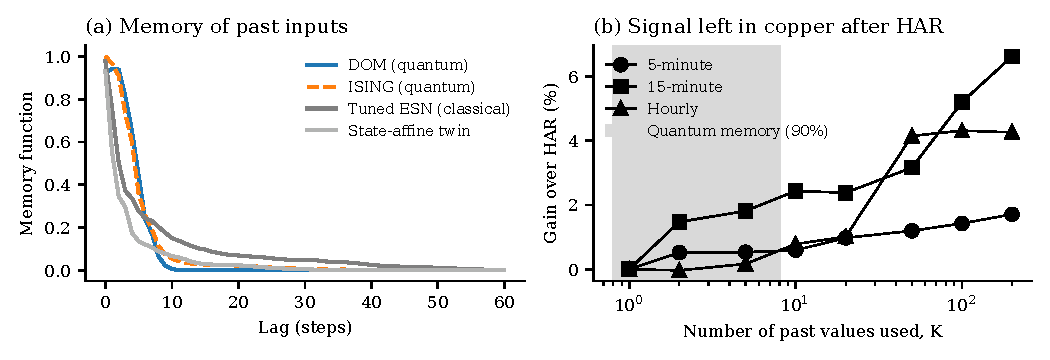
\includegraphics[width=\textwidth]{figs/sanda3.pdf}
\caption{(a) Linear memory function of the quantum reservoirs and of classical reservoirs on independent uniform inputs (median over seeds and settings). (b) Gain over HAR of a ridge regression on the last $K$ values of copper log realized variance, test years 2023--2025; the shaded band marks the quantum reservoirs' 90\% memory.}
\label{fig:mech}
\end{figure*}

\subsection{When Can a Quantum Reservoir Gain? A Positive Control}
\label{sec:res-map}
The validity check passed: the teacher's own circuit beat the best classical model detectably in three quantum-generated cells, by up to 3.7\% (ratio 0.9630). Quantum reservoirs with a different circuit never beat the validation-selected classical model in any of the 50 cells, including cells generated by quantum reservoirs of their own family (Fig.~\ref{fig:map}). They were detectably worse on short-memory data with three-way products (ratios 1.056 to 1.191). In the cells where the best classical model beats HAR by about as much as the single-input networks do on copper, every quantum comparison shows no detectable difference.

\begin{figure*}[t]
\centering
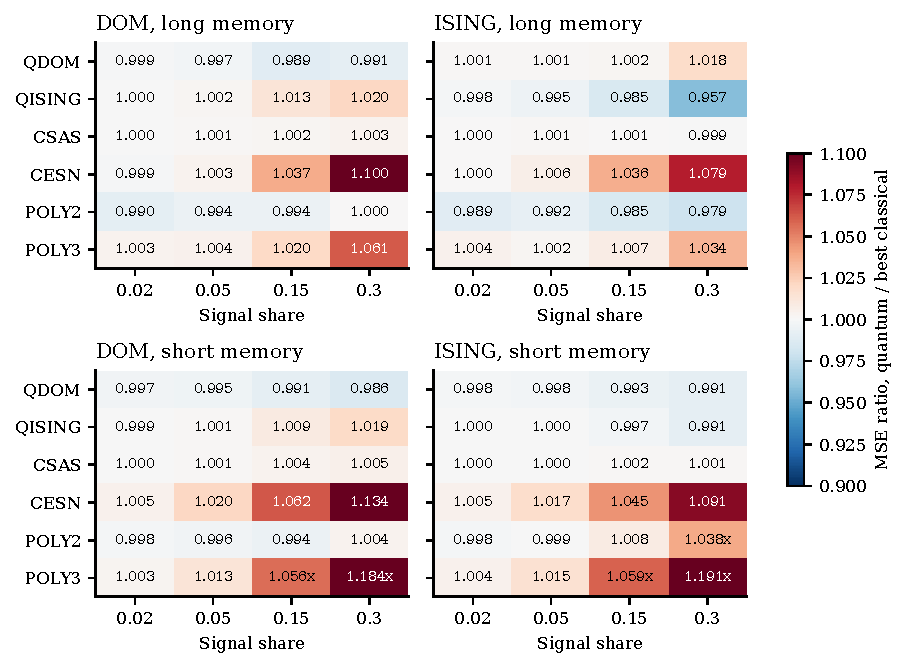
\includegraphics[width=0.85\textwidth]{figs/sanda4.pdf}
\caption{Synthetic positive control: loss ratio of each quantum reservoir to the validation-selected classical model, geometric mean over 10 datasets per cell, by teacher and signal share. ** meaningful edge, * detectable below band, x detectably worse.}
\label{fig:map}
\end{figure*}

\subsection{Earlier Registered Tests on Daily Copper}
\label{sec:res-earlier}
Before the intraday study, we tested a different reservoir on daily copper, each test registered in a hashed file before it was run. QRC\_angle is a six-qubit random circuit (layers of RX, RY and RZ rotations followed by a ring of CZ gates) simulated exactly. It reads the standardized log range variance over 1, 5 and 22 days, for today and yesterday, through an arctan angle encoding, and returns 21 features: six single-qubit and fifteen two-qubit $Z$ expectations. The readout adds these features to HAR-style inputs and is trained with the QLIKE loss; the number of layers and the input scale are tuned on validation years. The data are daily COMEX copper futures prices from Yahoo Finance with 17 rolling one-year test blocks from 2008 to 2024 (4,257 test days), and the target is the log of the mean daily variance over the next five days. The controls are a 21-unit echo state network, 21 tanh random features (RandFeat), the same circuit without CZ gates (QRC\_noent), exact trigonometric bases of degree 2 and 4 (Basis2, Basis4), random projections of the same size (RandProj), classical cosine features on the reservoir's input angles (TrigFeat), and a trained quantum LSTM (QLSTMT) \cite{chen2020}. Losses are QLIKE; a ratio is \emph{equivalent} when its 95\% interval lies inside $\pm3\%$ and \emph{inconclusive} when the interval contains 1 but leaves the band.

Table~\ref{tab:earlier} gives the results. The reservoir does not beat its matched echo state network (1.015, Holm $p=0.67$) or HAR (0.990, inconclusive), and it is equivalent to tanh random features. An exact degree-2 trigonometric basis reproduces the one-layer reservoir (0.9999); deeper circuits gain 2\% over a degree-4 basis but no more than a random projection of the same size. Classical cosine features match the reservoir, although this control was designed after the tie was known. Removing the entangling gates changes the error by about 1\%. The trained quantum LSTM is 8.9\% worse than a classical LSTM of matched size (Holm $p=0.002$).

No niche appears either. With 50 to 1,000 training days the tuned reservoir against the echo state network gives ratios from 0.961 to 1.018, none significant after Holm ($p\geq0.39$). In calm years the reservoir is 6\% worse than the echo state network (Holm $p=0.069$); in turbulent years the two are indistinguishable (0.998, interval 0.932 to 1.063). Adding lagged VIX, crude-oil and dollar-index variance as inputs makes the reservoir worse, not better (1.048 against a multivariate echo state network). Finally, we measured the 2024 test features of the tuned one-layer circuit on the \emph{ibm\_fez} processor (2000 shots, no error mitigation, one seed), keeping the readout trained on exact features. The QLIKE ratio of hardware to simulator is 1.0013 (interval 0.9926 to 1.0099, equivalent) with a mean absolute feature error of 0.030. This shallow circuit is robust to hardware noise, but robustness is not an advantage.

\begin{table}[t]
\caption{Earlier Registered Tests on Daily Copper, 2008--2024}
\label{tab:earlier}
\centering
\begin{tabular}{lcc}
\hline
Comparison & Ratio [95\% CI] & Verdict \\
\hline
\multicolumn{3}{l}{\textit{Against classical models}} \\
QRC\_angle / ESN & 1.015 [0.974, 1.056] & incon. \\
QRC\_angle / HAR & 0.990 [0.970, 1.010] & incon. \\
QRC\_angle / RandFeat & 1.013 [1.000, 1.025] & equiv. \\
QLSTMT / LSTM & 1.089 [1.039, 1.138] & worse \\
\multicolumn{3}{l}{\textit{Is the reservoir a classical feature map?}} \\
QRC\_L1 / Basis2 & 1.000 [0.983, 1.017] & equiv. \\
QRC\_L2 / Basis4 & 0.980 [0.962, 0.997] & better$^\mathrm{h}$ \\
QRC\_L2 / RandProj & 1.004 [0.997, 1.011] & equiv. \\
TrigFeat / QRC\_angle & 0.985 [0.976, 0.995] & equiv. \\
QRC\_angle / QRC\_noent & 1.011 [1.005, 1.018] & equiv. \\
\multicolumn{3}{l}{\textit{Possible niches}} \\
Calm years, / ESN & 1.060 [1.004, 1.115] & worse$^\mathrm{h}$ \\
Turbulent years, / ESN & 0.998 [0.932, 1.063] & incon. \\
Multivariate, / ESN & 1.048 [1.005, 1.091] & worse$^\mathrm{h}$ \\
Hardware / simulator & 1.001 [0.993, 1.010] & equiv. \\
\hline
\multicolumn{3}{p{7.6cm}}{\footnotesize QLIKE ratios; below 1 favors the first model. $^\mathrm{h}$Interval excludes 1, but the difference is not significant after Holm correction (Holm $p$ 0.068 to 0.116). The long daily reservoir registration predates its prediction files by local file timestamps only, and the QLSTMT registration has no stored hash.}\\
\end{tabular}
\end{table}

The same reservoir design was also run on the intraday copper data of Section~\ref{sec:data}, with eight qubits and eight standardized inputs (returns, log realized variance and log volume, current and lagged) and 36 features (8 single-qubit and 28 two-qubit $Z$ expectations), against a 36-unit echo state network and 36 classical cosine features. Table~\ref{tab:ownqrc} shows that it stays within 0.5\% of both controls in the rolling years and within 1\% in the held-out year; every interval lies inside the $\pm3\%$ band, so the registered edge rule was not met on any grid. On daily Databento copper (ten test years, 2015 to 2024) it is inconclusive against the echo state network (1.022, Holm $p=0.94$) and level with the cosine features (1.000). The project's own reservoir thus behaves like the classical feature maps it resembles, at every frequency we tried.

\begin{table}[t]
\caption{The Angle-Encoded Reservoir on Intraday Copper (MSE Ratios)}
\label{tab:ownqrc}
\centering
\begin{tabular}{lccc}
\hline
Comparison & 5 min & 15 min & 60 min \\
\hline
\multicolumn{4}{l}{\textit{Rolling test years 2013--2025}} \\
QRC / ESN & 1.0046 & 0.9984 & 0.9953 \\
QRC / TrigFeat & 1.0041 & 1.0016 & 0.9970 \\
\multicolumn{4}{l}{\textit{Held-out 2026}} \\
QRC / TrigFeat & 1.0054 & 1.0041 & 1.0075 \\
\hline
\multicolumn{4}{p{7.6cm}}{\footnotesize Tuned configuration at 15 and 60 minutes; the 5-minute grid was run only in the fixed configuration. All 95\% intervals lie inside $\pm1.3\%$ of 1.}\\
\end{tabular}
\end{table}

Fig.~\ref{fig:spec} pools every quantum-versus-classical comparison made on copper in this study: 1,120 specifications over three quantum reservoirs (DOM, ISING and QRC), four frequencies from 5 minutes to daily, rolling and held-out years, and several references. The median ratio is 0.9999 (5th to 95th percentile 0.955 to 1.039). Against matched reservoirs and classical twins, none of 600 specifications lies below the $-3\%$ band. Against networks with more inputs, the quantum reservoir is worse in all 180 intraday specifications. All 14 specifications below the band are daily rolling-year comparisons of DOM or ISING with single-input networks, which are weak at daily frequency (a single-input LSTM is 4\% worse than HAR there), and none comes from a held-out year. The specifications share data and models and their intervals are not corrected for multiplicity, so the curve is descriptive.

\begin{figure*}[t]
\centering
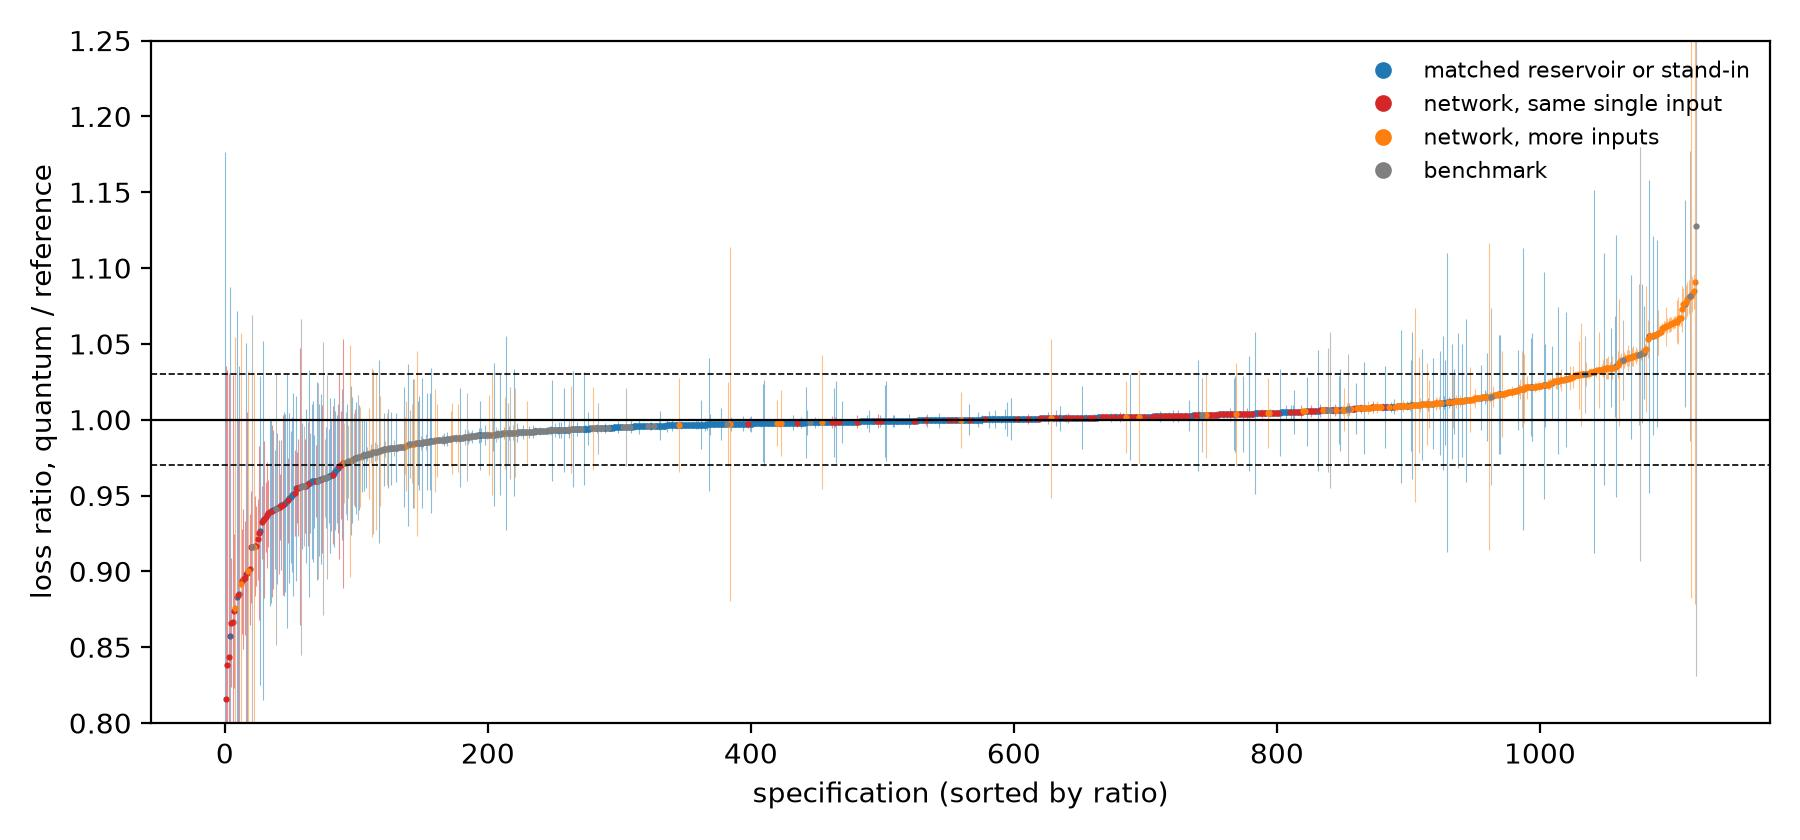
\includegraphics[width=\textwidth]{figs/sanda7.pdf}
\caption{Specification curve over 1,120 quantum-versus-classical comparisons on copper, sorted by loss ratio, with raw 95\% intervals. Colors mark the type of classical reference; dashed lines mark the $\pm3\%$ band.}
\label{fig:spec}
\end{figure*}

\subsection{Publicly Pre-Registered Held-Out Test on Gold and Silver}
\label{sec:res-heldout}
The registration \cite{osf2026} fixed three predictions over six market and frequency cells. All three were supported (Tables~\ref{tab:heldout} and~\ref{tab:heldout23}, Fig.~\ref{fig:heldout}).

\emph{R1, no quantum edge.} None of the 24 comparisons of DOM or ISING with LIN200 or LSTM1 shows a meaningful edge. The quantum reservoirs are detectably worse than LSTM1 in 9 of 12 comparisons (ratios 1.0009 to 1.0054) and not different in the remaining 3 (hourly). They are detectably worse than LIN200 at 15 and 60 minutes in all 8 comparisons (1.0042 to 1.0199) and slightly better at 5 minutes (0.9945 to 0.9963), well inside the $\pm3\%$ band.

\emph{R2, signal beyond memory.} $K^*$ is 200 in five cells and 100 in one (silver, hourly), far above the reservoirs' memory of 8 steps or less.

\emph{R3, no information beyond a same-memory classical model.} Combinations of LIN200 with DOM and with ESNb\_t, each with one weight chosen on the previous test year, differ by at most 0.18\% (ratios 0.9988 to 1.0018), and all six 90\% intervals lie inside the registered margins.

\emph{Further checks.} In the held-out 2026 blocks, no comparison shows a meaningful edge (8 of 24 detectably worse, 16 not different). Restricted to years never examined at any frequency (gold 2018--2019, silver 2013--2019), R1 still holds; R3 passes in four of six cells, and the two misses (silver at 5 and 60 minutes) have the quantum combination worse. Table~\ref{tab:heldcheck} gives both checks.

\begin{table}[t]
\caption{Held-Out Test, R1: Loss Ratios of the Quantum Reservoirs}
\label{tab:heldout}
\centering
\setlength{\tabcolsep}{3pt}
\begin{tabular}{llcccc}
\hline
& & \multicolumn{2}{c}{vs. LIN200} & \multicolumn{2}{c}{vs. LSTM1} \\
Asset & Freq. & DOM & ISING & DOM & ISING \\
\hline
Gold & 5 min & 0.9955$^\mathrm{b}$ & 0.9945$^\mathrm{b}$ & 1.0040$^\mathrm{w}$ & 1.0030$^\mathrm{w}$ \\
Gold & 15 min & 1.0049$^\mathrm{w}$ & 1.0042$^\mathrm{w}$ & 1.0016$^\mathrm{w}$ & 1.0009$^\mathrm{w}$ \\
Gold & 60 min & 1.0180$^\mathrm{w}$ & 1.0159$^\mathrm{w}$ & 1.0027$^\mathrm{w}$ & 1.0006 \\
Silver & 5 min & 0.9963$^\mathrm{b}$ & 0.9960$^\mathrm{b}$ & 1.0054$^\mathrm{w}$ & 1.0051$^\mathrm{w}$ \\
Silver & 15 min & 1.0102$^\mathrm{w}$ & 1.0099$^\mathrm{w}$ & 1.0027$^\mathrm{w}$ & 1.0023$^\mathrm{w}$ \\
Silver & 60 min & 1.0199$^\mathrm{w}$ & 1.0183$^\mathrm{w}$ & 1.0010 & 0.9994 \\
\hline
\multicolumn{6}{p{7.8cm}}{\footnotesize Rolling test years 2013--2025 (LIN200 at 60 minutes: 2015--2025). $^\mathrm{w}$Detectably worse. $^\mathrm{b}$Detectable, below band. Unmarked: no detectable difference. Meaningful edges: 0 of 24, so R1 is supported. Every 95\% interval is narrower than $\pm0.6\%$. Registration DOI 10.17605/OSF.IO/YJ6W4.}\\
\end{tabular}
\end{table}

\begin{table}[t]
\caption{Held-Out Test, R2 and R3}
\label{tab:heldout23}
\centering
\setlength{\tabcolsep}{3pt}
\begin{tabular}{llcc}
\hline
Asset & Freq. & R2: $K^*$ & R3: A/B [90\% interval] \\
\hline
Gold & 5 min & 200 & 1.0007 [1.0005, 1.0010] \\
Gold & 15 min & 200 & 0.9988 [0.9985, 0.9990] \\
Gold & 60 min & 200 & 0.9993 [0.9984, 1.0002] \\
Silver & 5 min & 200 & 1.0018 [1.0014, 1.0021] \\
Silver & 15 min & 200 & 0.9993 [0.9991, 0.9995] \\
Silver & 60 min & 100 & 1.0018 [1.0004, 1.0031] \\
\hline
\multicolumn{4}{p{7.8cm}}{\footnotesize R2 passes if $K^*>8$: 6 of 6. R3: loss ratio of the combination of LIN200 with DOM (A) to its combination with ESNb\_t (B); passes if the 90\% interval lies inside $\pm0.25\%$ at 5 minutes or $\pm0.5\%$ at 15 and 60 minutes: 6 of 6.}\\
\end{tabular}
\end{table}

\begin{figure*}[t]
\centering
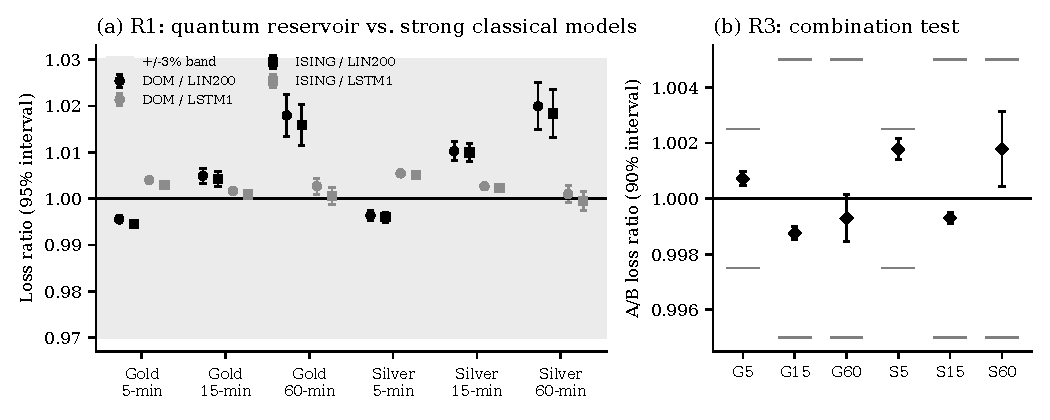
\includegraphics[width=\textwidth]{figs/sanda6.pdf}
\caption{Held-out test on gold and silver. (a) R1: loss ratios of DOM and ISING to LIN200 and LSTM1 with 95\% intervals; the shaded band is $\pm3\%$. (b) R3: loss ratio of the combination with DOM to the combination with a same-memory classical reservoir, with 90\% intervals; the short lines mark the registered margins.}
\label{fig:heldout}
\end{figure*}

\begin{table}[t]
\caption{Further Checks on Gold and Silver (Not Decision Rules)}
\label{tab:heldcheck}
\centering
\setlength{\tabcolsep}{2.5pt}
\begin{tabular}{lccccc}
\hline
& \multicolumn{2}{c}{vs. LIN200} & \multicolumn{2}{c}{vs. LSTM1} & \\
Cell & DOM & ISING & DOM & ISING & R3 A/B \\
\hline
\multicolumn{6}{l}{\textit{Held-out 2026}} \\
Gold 5 min & 1.0047 & 1.0027 & 1.0100$^\mathrm{w}$ & 1.0080$^\mathrm{w}$ & -- \\
Gold 15 min & 1.0207$^\mathrm{w}$ & 1.0477$^\mathrm{w}$ & 1.0103$^\mathrm{w}$ & 1.0369 & -- \\
Gold 60 min & 1.0044 & 1.0101 & 1.0030 & 1.0086 & -- \\
Silver 5 min & 1.0047 & 1.0015 & 1.0020 & 0.9988 & -- \\
Silver 15 min & 1.0289$^\mathrm{w}$ & 1.0684$^\mathrm{w}$ & 1.0054$^\mathrm{w}$ & 1.0439 & -- \\
Silver 60 min & 0.9809 & 1.0004 & 0.9979 & 1.0177 & -- \\
\multicolumn{6}{l}{\textit{Never-examined years (gold 2018--2019, silver 2013--2019)}} \\
Gold 5 min & 0.9953$^\mathrm{b}$ & 0.9952$^\mathrm{b}$ & 1.0040$^\mathrm{w}$ & 1.0039$^\mathrm{w}$ & 1.0018 \\
Gold 15 min & 1.0056$^\mathrm{w}$ & 1.0046$^\mathrm{w}$ & 1.0006 & 0.9996 & 1.0004 \\
Gold 60 min & 0.9966 & 0.9943 & 1.0016 & 0.9993 & 0.9992 \\
Silver 5 min & 0.9902$^\mathrm{b}$ & 0.9894$^\mathrm{b}$ & 1.0035$^\mathrm{w}$ & 1.0027$^\mathrm{w}$ & 1.0029$^\mathrm{m}$ \\
Silver 15 min & 0.9962$^\mathrm{b}$ & 0.9960$^\mathrm{b}$ & 1.0012$^\mathrm{w}$ & 1.0009$^\mathrm{w}$ & 0.9996 \\
Silver 60 min & 0.9833$^\mathrm{b}$ & 0.9803$^\mathrm{b}$ & 1.0022 & 0.9992 & 1.0034$^\mathrm{m}$ \\
\hline
\multicolumn{6}{p{7.8cm}}{\footnotesize $^\mathrm{w}$Detectably worse. $^\mathrm{b}$Detectable, below band. Unmarked: no detectable difference. $^\mathrm{m}$Outside the R3 margin, with the quantum combination worse. No ratio is a meaningful edge. R3 was not part of the 2026 check.}\\
\end{tabular}
\end{table}

\subsection{How Evaluation Choices Create an Apparent Quantum Advantage}
\label{sec:res-choices}
To show how the copper result could be reported as a quantum advantage, we re-enacted six evaluation choices on the saved copper forecasts without refitting any model (Table~\ref{tab:factors}). Under a protocol, the researcher reports the option that makes the quantum model look best among the options left open. For a protocol $\pi$ with open options $O(\pi)$ and loss ratios $R_o$, the apparent advantage of a researcher who reports the best option, and of one who picks at random, is
\begin{equation}
A_{\mathrm{best}}(\pi)=1-\min_{o\in O(\pi)}R_o,
\label{eq:adv}
\end{equation}
\begin{equation}
A_{\mathrm{rand}}(\pi)=1-\exp\Big(\tfrac{1}{|O(\pi)|}\textstyle\sum_{o}\log R_o\Big).
\label{eq:advrand}
\end{equation}

\begin{table}[t]
\caption{Evaluation Choices Re-Enacted on Saved Copper Forecasts}
\label{tab:factors}
\centering
\begin{tabular}{p{1.45cm}p{2.95cm}p{2.95cm}}
\hline
Choice & Sound value & Choice after seeing test results \\
\hline
Seeds & mean of 10 seeds & best 3 of 10 seeds \\
Test year & all years pooled & best single year \\
Frequency & geometric mean over grids & best grid \\
Loss & squared error & best of squared error, absolute error, quasi-likelihood (QLIKE) \\
Quantum model & DOM, fixed in advance & better of DOM and ISING \\
Reference & classical model best in the previous year & untuned 28-unit echo state network \\
\hline
\end{tabular}
\end{table}

Under the sound protocol, DOM is 3.5\% worse than the classical model that was best in the previous year (ratio 1.0349; that model was LSTM or GRU in 29 of 36 grid-years). With the five choices that select on test results, DOM looks 19.8\% better; with all six, 6.8\% better (Fig.~\ref{fig:budget}). Shapley values \cite{shapley1953} attribute most of the swing to the loss (56\%) and the test year (44\%). A researcher who picks the same options at random gains almost nothing ($A_{\mathrm{rand}}=-2.6\%$ and $+0.4\%$): the apparent advantage comes from selecting on test results. Choosing the best test year alone produces a median apparent gain of about 5.5\% even between two equal models, estimated by swapping whole test years between them. Table~\ref{tab:null} compares each choice with that year-block null: choosing the loss, the quantum model or the seeds produces more apparent gain than chance, choosing the test year or frequency produces gains of the size that chance alone would give, and all five together exceed the null.

\begin{table}[t]
\caption{Apparent Gain of Each Choice Against a Year-Block Null (Log Points)}
\label{tab:null}
\centering
\begin{tabular}{lccc}
\hline
Choice & Observed & Null median & Null 95th pct. \\
\hline
Seeds & 0.11 & 0.01 & 0.07 \\
Test year & 3.09 & 5.66 & 7.26 \\
Frequency & 1.15 & 0.74 & 1.74 \\
Loss & 4.80 & 3.10 & 4.14 \\
Quantum model & 0.18 & 0.02 & 0.16 \\
All five & 25.54 & 20.96 & 23.70 \\
\hline
\multicolumn{4}{p{7.6cm}}{\footnotesize Gain over the sound protocol, 100 times the change in log loss ratio. Null: 1000 random exchanges of whole test years between DOM and the reference.}\\
\end{tabular}
\end{table}

Seeds alone can also decide a comparison. On hourly copper over a two-year span, a trained quantum long short-term memory network (QLSTM) \cite{chen2020} and a parameter-matched LSTM were each run with 50 seeds; over all seeds the QLSTM is 2.2\% worse (ratio 1.0222). A researcher who runs one seed per model sees the QLSTM ahead 13\% of the time; with three seeds 7\%, with ten 1\%, and with 25 never (Fig.~\ref{fig:null}(b)).

 On a second panel of 11 commodity futures with six quantum models, the same choices produced apparent advantages of up to 86\%, with the asset choice and a weak reference contributing most. Table~\ref{tab:panel} gives the details. The registered replication rule, that the loss and the test window would again be the two largest contributions, failed: which choice matters most depends on the dataset. On this panel the sound protocol itself shows the quantum model 7.2\% better, but the result is driven by two assets (palladium and platinum) on which the classical reference failed, and the quantum model is worse than its reference on 7 of the 11 assets.

\begin{table}[t]
\caption{Second Dataset: 11 Commodity Futures, Hourly}
\label{tab:panel}
\centering
\begin{tabular}{lcc}
\hline
Choice & Apparent advantage & Shapley share \\
\hline
Asset & +68.1\% & 41\% \\
Test quarter & +33.0\% & 22\% \\
Seeds & +14.9\% & 3\% \\
Loss & +13.8\% & 3\% \\
Quantum model & +12.9\% & 1\% \\
Weak reference & -- & 30\% \\
All five selection choices & +86.0\% & -- \\
\hline
\multicolumn{3}{p{7.6cm}}{\footnotesize Six quantum models; 17-month test period. Apparent advantage of a researcher who reports the best option of each choice alone, and of all five together.}\\
\end{tabular}
\end{table}

These choices are common. We assembled QML papers that forecast a time series and compare quantum with classical models, obtained full text from arXiv, open-access publisher copies and other open repositories, and coded 52 of them against 12 pitfalls with written rules; a pitfall was coded as present or absent only when the text allowed it, and otherwise as not reported. Among the 52 papers, coded by one coder (Fig.~\ref{fig:prev}), 85\% lack a statistical test or a multiple-testing correction (44 of 52), 82\% use one seed or no repeated runs (42 of 51), 77\% use a single train and test split (34 of 44), and 76\% have no naive or strong benchmark (39 of 51). A further 63\% report only level metrics such as root mean squared error with no naive comparison (22 of 35), and the median paper has four pitfalls.

\begin{figure*}[t]
\centering
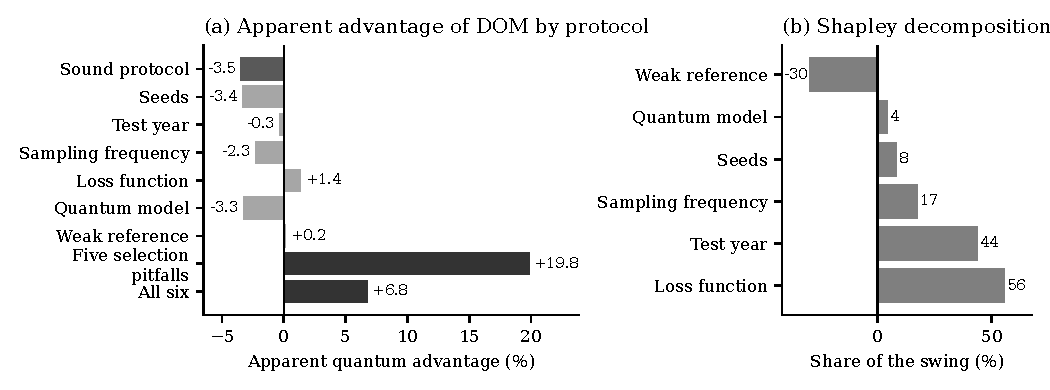
\includegraphics[width=\textwidth]{figs/sanda1.pdf}
\caption{(a) Apparent advantage of DOM on copper under the sound protocol, under each choice alone, under the five choices that select on test results, and under all six. (b) Shapley shares of the change in log ratio from the sound protocol to all six choices.}
\label{fig:budget}
\end{figure*}

\begin{figure*}[t]
\centering
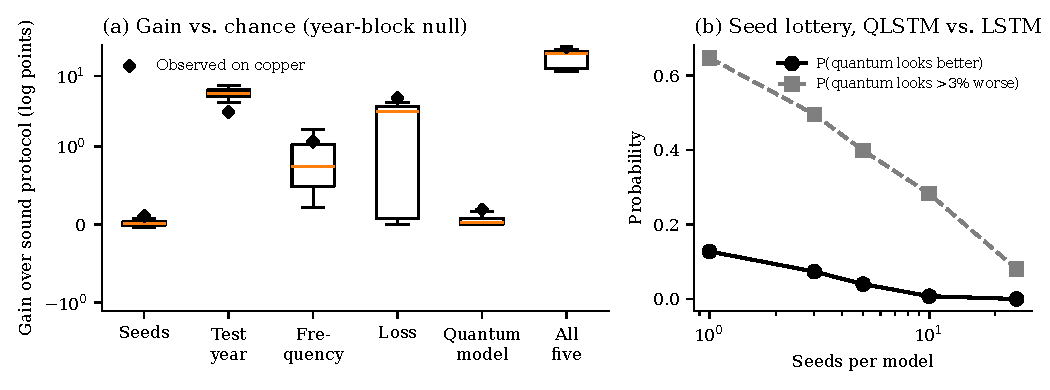
\includegraphics[width=\textwidth]{figs/sanda2.pdf}
\caption{(a) Apparent gain of each evaluation choice on copper (diamonds) against its distribution under the year-block null (boxes: median and quartiles; whiskers: 5th and 95th percentiles). (b) Probability that a quantum LSTM looks better than an LSTM, or more than 3\% worse, when each is run with a given number of random seeds; over 50 seeds the quantum model is 2.2\% worse.}
\label{fig:null}
\end{figure*}

\begin{figure}[t]
\centering
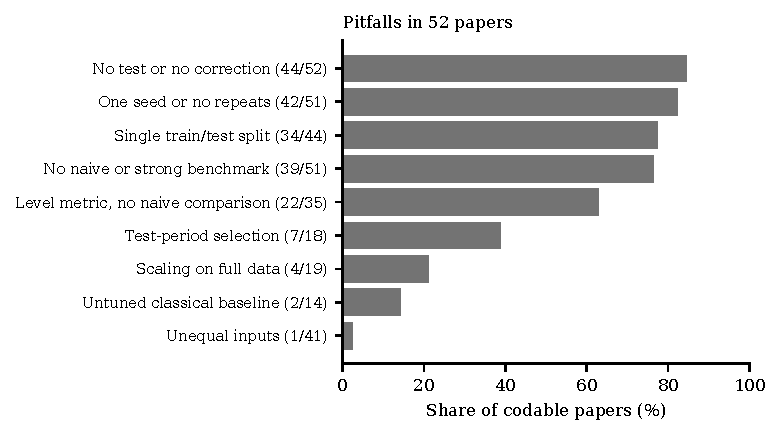
\includegraphics[width=\columnwidth]{figs/sanda5.pdf}
\caption{Share of 52 published QML forecasting papers with each evaluation pitfall, among papers where it could be coded (counts in brackets); single coder.}
\label{fig:prev}
\end{figure}

\section{Discussion}
\label{sec:discussion}

\subsection{Memory, Not Quantumness, Limits These Reservoirs}
The quantum reservoirs fail on copper for a reason that does not depend on quantum effects: they forget the past within a few steps, and the information that a forecaster can still use after HAR lies hundreds of steps back. A linear model that reads those lags directly does better, and a classical reservoir of the same memory adds as much information in combination as the quantum one. The positive control shows that a quantum reservoir can gain only when it is the very circuit that produced the data, and then by less than 4\%. The held-out test confirms all of this on two assets whose minute-level data the authors had not loaded. For volatility forecasting, matching a model's memory to the data's lag structure is the first requirement; a quantum design is worth testing only if its memory meets it.

\subsection{What Would a Useful Quantum Reservoir Need?}
The lag probe sets a concrete target. At 5 minutes, 200 bins cover about 17 hours of trading; at 15 minutes, about two trading days; and at 60 minutes, $K^*=50$ covers about two days. The tuned echo state network reaches 32 steps, and the quantum reservoirs 5 to 8. A quantum reservoir that is to compete must therefore keep information for tens to hundreds of steps while still adding a nonlinear transformation that a linear model cannot supply. Several designs could lengthen memory: encoding several lagged inputs at once on separate qubits, resetting fewer qubits per step or resetting them only partially, feeding measured outputs back as inputs, and tuning dissipation to the time scale of the data. The combination test (R3) adds a second requirement: whatever such a reservoir computes must carry information that a same-memory classical reservoir does not, because on gold and silver the quantum and classical reservoirs added the same amount to the linear model. A practical design would therefore pair a long-lag linear component with a quantum reservoir and test the reservoir's contribution against a classical twin of equal memory.

\subsection{Reading Claims of Quantum Advantage}
The same copper forecasts can be presented as a 20\% quantum advantage by choosing, after seeing test results, the loss, the test year, the frequency, the seeds and the quantum model. These choices appear in most published QML forecasting papers we coded. Claims of quantum advantage should state these choices in advance, compare against a strong linear benchmark and a same-memory classical reservoir, and, where possible, be confirmed on data that the authors have not examined.

\subsection{Relation to the Companion Audit}
The companion audit \cite{companion} examined one published claim on its authors' monthly data and found that the reported edge depended on choices that coincide with the test period. The present study reaches a consistent conclusion from the opposite direction: it starts from a sound protocol on new, high-frequency data, explains the absence of an edge by a measurable property of the models, and confirms that explanation on data the authors had not loaded. Together, the two studies suggest that the evidence for quantum advantage in volatility forecasting is weaker than the published claims imply.

\subsection{Practical Checklist}
Table~\ref{tab:checklist} lists the checks we recommend for any claim that a quantum model forecasts financial time series better than classical ones, with the evidence from this study that motivates each.

\begin{table}[t]
\caption{Checks for a Quantum Forecasting Claim}
\label{tab:checklist}
\centering
\begin{tabular}{p{3.2cm}p{4.1cm}}
\hline
Check & Motivation in this study \\
\hline
Compare with HAR and a long-lag linear model & LIN200 beats every quantum reservoir at 15 and 60 minutes \\
Include a same-memory classical reservoir & twins match DOM at 5 minutes and in combination \\
Measure memory and the data's lag structure & 5--8 steps of memory against signal at 50--200 lags \\
Fix loss, test period, seeds and model in advance & choosing them after seeing results gives up to 20\% \\
Use several seeds & one seed reverses a 2.2\% deficit 13\% of the time \\
Confirm on unseen data with public predictions & all three predictions held on gold and silver \\
\hline
\end{tabular}
\end{table}

\subsection{Threats to Validity}
\textit{Internal validity.} The copper analyses were designed in sequence, so later steps were chosen with knowledge of earlier results; the public held-out test is the safeguard against this, and its predictions were derived from copper before the gold and silver data were bought. \textit{Construct validity.} Memory was measured on independent uniform inputs rather than on the distribution of copper volatility, and $K^*$ is measured with a linear probe, so nonlinear long-lag structure is not captured. \textit{External validity.} Two quantum designs with seven qubits, simulated without noise, and three metals from one exchange do not cover the space of quantum reservoirs or markets. \textit{Statistical conclusion validity.} With hundreds of thousands of test bins, differences far below the $\pm3\%$ band are detectable, which is why each result is classified by size as well as by significance.

\subsection{Limitations}
The held-out assets are two metals from the same exchange; gold and silver had been seen at daily and hourly frequency from another source, and in the never-examined years R3 passed in four of six cells. The intraday quantum reservoirs are small and simulated without hardware noise; only the shallow daily reservoir was run on a quantum processor, for one test year. The copper analyses were registered in sequence after earlier results, and several post-hoc readings are labelled as such (Appendix~\ref{app:deviations}). The evaluation-choice measurements assume a researcher who always picks the best-looking option and are an upper bound on what each choice produces. The prevalence coding was done by a single coder and has no inter-rater agreement.

\section{Conclusion}
\label{sec:conclusion}
On intraday copper volatility, two published quantum reservoir designs do not beat strong classical models or a 200-lag linear model, because their memory is far shorter than the lags at which the remaining signal lies. Three predictions derived from this result were registered publicly and all held on held-out gold and silver data. Evaluation choices made after seeing test results can still make the reservoirs look up to 20\% better, which is why such claims need fixed protocols, strong linear and same-memory baselines, and held-out confirmation. Future work should test quantum reservoirs whose memory is designed to reach long lags, for example with feedback or dissipation tuned to the data, and should test them on hardware.

\section*{Data and Code Availability}
The pre-registration of the held-out test, with SHA-256 hashes of every script, its addenda and its results, is public at doi:10.17605/OSF.IO/YJ6W4. Code, registration files with their hashes, and aggregate reports: \url{https://github.com/Janindu2204/qrc-commodity-memory}, archived as release v1.0 (commit 9b8cc8b) on Zenodo, doi: 10.5281/zenodo.24444166. The Databento market data are licensed and cannot be redistributed, and neither are forecasts derived from them; the repository includes scripts that rebuild every dataset from a licensed download. Daily series were downloaded from the Yahoo Finance chart interface.

\section*{Competing Interests}
The authors declare no competing interests.

\appendices

\section{Deviations From the Registrations}
\label{app:deviations}
\begin{enumerate}
\item \textit{Copper, sequential design.} The copper comparisons were registered in steps, each designed after the previous results, and a stop rule was relaxed for the memory analysis, the linear benchmark and a null distribution. These analyses are reported as disclosed exceptions.
\item \textit{Positive control.} The first run fed the planted signal back into the input, so the signal became constant in many datasets and the validity check failed; the corrected generator was registered before it ran, and both runs are reported in the repository.
\item \textit{Evaluation-choice null.} The first registered null, which swaps weeks, was too narrow; a year-block null was registered afterwards. The second panel's run was stopped before any result was printed to correct the units of the saved forecasts.
\item \textit{Memory threshold.} The rule for a no-memory control counted the current input as memory; split by lag, the control has no memory of past inputs.
\item \textit{An exploratory analysis was withdrawn.} A registered hypothesis that the spread of results across options predicts which choice creates most apparent advantage turned out to be nearly circular (pure noise passed it 98.5\% of the time) and is not used; a companion prediction of the exact size failed.
\item \textit{Daily copper tests.} The long daily reservoir registration is dated one day after the local timestamps of its own file, which predate the first prediction file by about an hour; no independent time stamp exists. The quantum LSTM comparison was registered without a stored hash. The TrigFeat control was designed after the reservoir was seen to tie the echo state network.
\item \textit{Held-out test.} The registered download script had a syntax error and was run with a one-line fix; the registration's answer that the data did not yet exist was corrected to ``existed but had not been accessed''; the run was paused, the computer restarted, and the run resumed with a launcher that runs only unfinished registered jobs; three jobs killed by lack of memory were re-run unchanged; the 60-minute LIN200 blocks for 2013 and 2014 were outside the registered window. All are posted as dated addenda on OSF.
\end{enumerate}

\section{Method Details}
\label{app:methods}
\textit{Evaluation choices.} Seeds: the 120 subsets of 3 of 10 seeds. Test year: the 12 years 2014--2025 (2013 only chooses the 2014 reference). Loss: squared and absolute error of log realized variance, and QLIKE, $L(x,\hat{x})=e^{x-\hat{x}}-(x-\hat{x})-1$, on the variance level \cite{patton2011}. Shapley values of the log ratio average each choice's effect over all orders in which the choices can be added. Nulls exchange the quantum and reference forecasts (every seed) in randomly selected weeks or whole years.

\textit{Positive control.} Inputs follow $x_{t+1}=b_1x_t+b_2\bar{x}^{(10)}_t+b_3\bar{x}^{(50)}_t+e_{t+1}$, $e_t\sim N(0,1)$, with $(b_1,b_2,b_3)=(0.35,0.35,0.25)$ or $(0.6,0,0)$, over 7000 steps after 500 burn-in steps. The teacher output is projected off $[1,x_t,\bar{x}^{(10)}_t,\bar{x}^{(50)}_t]$, scaled to unit variance, and added as $y_{t+1}=x_{t+1}+a\,g_t$ with $a=\sqrt{s/(1-s)}$. Training, validation and test steps are $t<4000$, $4024\le t<5000$ and $t\ge5024$.

\textit{Combination test (R3).} Each combination is $(1-w)\hat{x}^{\mathrm{LIN200}}+w\,\hat{x}^{Q}$ with $w\in\{0,0.05,\dots,1\}$ chosen by squared error on the previous test year; the margins are $\pm0.25\%$ at 5 minutes and $\pm0.5\%$ at 15 and 60 minutes, with 90\% Newey-West intervals.

\section*{Acknowledgment}
The authors used Claude (Anthropic), through the Claude Code tool (November 2026), as an assistant throughout this work. It drafted the analysis and simulation code, the registration files, the figure scripts and first drafts of all sections of the manuscript; it assisted with literature searches and reference checks against Crossref and arXiv; and an instance of it performed the full-text coding of the 52 papers in Fig.~\ref{fig:prev}. All study design decisions, registrations and interpretations were reviewed and approved by the authors. The authors reviewed all code, results, references and text, and take full responsibility for the content of this article.

\begin{thebibliography}{00}

\bibitem{li2026}Q. Li, C. Mukhopadhyay, A. Bayat, and A. Habibnia, ``Quantum reservoir computing for realized volatility forecasting,'' \emph{Phys. Rev. Res.}, vol. 8, no. 2, 2026, Art. no. 023028, doi: 10.1103/rbj7-4wnq.

\bibitem{pandey2026}T. Pandey, ``When classical baselines are tuned as carefully as the quantum model, does quantum reservoir computing still win?'' 2026, \emph{arXiv:2607.09905 [quant-ph]}.

\bibitem{maheshwari2026b}D. Maheshwari, G. Hellstern, M. Zaefferer, M. Braun, and T. D\"ohler, ``Quantum recurrent architectures for financial time series prediction,'' 2026, \emph{arXiv:2611.15298 [quant-ph]}.

\bibitem{fellner2026}T. Fellner, D. A. Kreplin, S. Tovey, and C. Holm, ``Quantum vs. classical: A comprehensive benchmark study for predicting time series with variational quantum machine learning,'' \emph{Mach. Learn.: Sci. Technol.}, vol. 7, no. 1, 2026, Art. no. 010501, doi: 10.1088/2632-2153/ae365f.

\bibitem{andersen2003}T. G. Andersen, T. Bollerslev, F. X. Diebold, and P. Labys, ``Modeling and forecasting realized volatility,'' \emph{Econometrica}, vol. 71, no. 2, pp. 579--625, 2003, doi: 10.1111/1468-0262.00418.

\bibitem{corsi2009}F. Corsi, ``A simple approximate long-memory model of realized volatility,'' \emph{J. Financ. Econometrics}, vol. 7, no. 2, pp. 174--196, 2009, doi: 10.1093/jjfinec/nbp001.

\bibitem{dambre2012}J. Dambre, D. Verstraeten, B. Schrauwen, and S. Massar, ``Information processing capacity of dynamical systems,'' \emph{Sci. Rep.}, vol. 2, 2012, Art. no. 514, doi: 10.1038/srep00514.

\bibitem{bowles2024}J. Bowles, S. Ahmed, and M. Schuld, ``Better than classical? The subtle art of benchmarking quantum machine learning models,'' 2024, \emph{arXiv:2403.07059 [quant-ph]}.

\bibitem{white2000}H. White, ``A reality check for data snooping,'' \emph{Econometrica}, vol. 68, no. 5, pp. 1097--1126, 2000, doi: 10.1111/1468-0262.00152.

\bibitem{domingo2026}L. Domingo, M. Grande, G. Carlo, F. Borondo, and J. Borondo, ``Optimal quantum reservoir computing for market forecasting: An application to fight food price crises,'' \emph{Eng. Appl. Artif. Intell.}, vol. 182, 2026, Art. no. 115854, doi: 10.1016/j.engappai.2026.115854.

\bibitem{companion}S. J. I. Sandanayaka, M. Edirisooriya, and A. Aponso, ``Does a quantum reservoir computing advantage in volatility forecasting survive honest evaluation? A pre-registered audit,'' manuscript, 2026. Code and data: doi: 10.5281/zenodo.24444274.

\bibitem{martinezpena2023}R. Mart\'inez-Pe\~na and J.-P. Ortega, ``Quantum reservoir computing in finite dimensions,'' \emph{Phys. Rev. E}, vol. 107, no. 3, 2023, Art. no. 035306, doi: 10.1103/PhysRevE.107.035306.

\bibitem{schutte2025}N.-E. Sch\"utte, N. G\"otting, H. M\"untinga, M. List, D. Brunner, and C. Gies, ``Expressivity of quantum reservoir computers,'' 2025, \emph{arXiv:2501.15528 [quant-ph]}.

\bibitem{nguyen2026}P. H. Nguyen and D. Soh, ``Quantum-Fisher-information-aware optimization yields a quantum reservoir advantage over tuned classical reservoirs,'' 2026, \emph{arXiv:2610.14454 [quant-ph]}.

\bibitem{jaeger2004}H. Jaeger and H. Haas, ``Harnessing nonlinearity: Predicting chaotic systems and saving energy in wireless communication,'' \emph{Science}, vol. 304, no. 5667, pp. 78--80, 2004, doi: 10.1126/science.1091277.

\bibitem{maheshwari2026a}D. Maheshwari, G. Hellstern, M. Zaefferer, M. Braun, and T. D\"ohler, ``Learning temporal patterns in financial time series: A comparative study of quantum LSTM and quantum reservoir computing,'' 2026, \emph{arXiv:2605.02656 [quant-ph]}.

\bibitem{shen2026}J. Shen, ``Quantum kernels and the cross-section of stock returns: Anatomy of a vanishing advantage,'' 2026, \emph{arXiv:2607.20168 [q-fin.PR]}.

\bibitem{islam2026}M. R. Islam, ``Benchmarking quantum machine learning for power-system attack detection: Evaluation choices decide the outcome before the models do,'' 2026, \emph{arXiv:2608.15617 [cs.LG]}.

\bibitem{bouthillier2021}X. Bouthillier \emph{et al.}, ``Accounting for variance in machine learning benchmarks,'' in \emph{Proc. Mach. Learn. Syst.}, 2021, \emph{arXiv:2103.03098 [cs.LG]}.

\bibitem{kapoor2023}S. Kapoor and A. Narayanan, ``Leakage and the reproducibility crisis in machine-learning-based science,'' \emph{Patterns}, vol. 4, no. 9, 2023, Art. no. 100804, doi: 10.1016/j.patter.2023.100804.

\bibitem{arp2022}D. Arp \emph{et al.}, ``Dos and don'ts of machine learning in computer security,'' in \emph{Proc. USENIX Secur. Symp.}, 2022, \emph{arXiv:2010.09470 [cs.CR]}.

\bibitem{hansen2005}P. R. Hansen, ``A test for superior predictive ability,'' \emph{J. Bus. Econ. Statist.}, vol. 23, no. 4, pp. 365--380, 2005, doi: 10.1198/073500105000000063.

\bibitem{harvey2016}C. R. Harvey, Y. Liu, and H. Zhu, ``... and the cross-section of expected returns,'' \emph{Rev. Financ. Stud.}, vol. 29, no. 1, pp. 5--68, 2016, doi: 10.1093/rfs/hhv059.

\bibitem{bailey2014}D. H. Bailey, J. M. Borwein, M. L\'opez de Prado, and Q. J. Zhu, ``Pseudo-mathematics and financial charlatanism: The effects of backtest overfitting on out-of-sample performance,'' \emph{Notices Amer. Math. Soc.}, vol. 61, no. 5, pp. 458--471, 2014, doi: 10.1090/noti1105.

\bibitem{simonsohn2020}U. Simonsohn, J. P. Simmons, and L. D. Nelson, ``Specification curve analysis,'' \emph{Nat. Hum. Behav.}, vol. 4, no. 11, pp. 1208--1214, 2020, doi: 10.1038/s41562-020-0912-z.

\bibitem{hochreiter1997}S. Hochreiter and J. Schmidhuber, ``Long short-term memory,'' \emph{Neural Comput.}, vol. 9, no. 8, pp. 1735--1780, 1997, doi: 10.1162/neco.1997.9.8.1735.

\bibitem{cho2014}K. Cho \emph{et al.}, ``Learning phrase representations using RNN encoder-decoder for statistical machine translation,'' 2014, \emph{arXiv:1406.1078 [cs.CL]}.

\bibitem{osf2026}S. J. I. Sandanayaka, ``Pre-registration of a held-out-asset test on gold and silver futures,'' OSF Registries, 2026, doi: 10.17605/OSF.IO/YJ6W4.

\bibitem{newey1987}W. K. Newey and K. D. West, ``A simple, positive semi-definite, heteroskedasticity and autocorrelation consistent covariance matrix,'' \emph{Econometrica}, vol. 55, no. 3, pp. 703--708, 1987, doi: 10.2307/1913610.

\bibitem{holm1979}S. Holm, ``A simple sequentially rejective multiple test procedure,'' \emph{Scand. J. Statist.}, vol. 6, no. 2, pp. 65--70, 1979, doi: 10.2307/4615733.

\bibitem{chen2020}S. Y.-C. Chen, S. Yoo, and Y.-L. L. Fang, ``Quantum long short-term memory,'' 2020, \emph{arXiv:2009.01783 [quant-ph]}.

\bibitem{shapley1953}L. S. Shapley, ``A value for $n$-person games,'' in \emph{Contributions to the Theory of Games}, vol. II, H. W. Kuhn and A. W. Tucker, Eds. Princeton, NJ, USA: Princeton Univ. Press, 1953, pp. 307--318, doi: 10.1515/9781400881970-018.

\bibitem{patton2011}A. J. Patton, ``Volatility forecast comparison using imperfect volatility proxies,'' \emph{J. Econometrics}, vol. 160, no. 1, pp. 246--256, 2011, doi: 10.1016/j.jeconom.2010.03.034.

\end{thebibliography}

\begin{IEEEbiographynophoto}{Sandanayakage Janindu Indira Sandanayaka}
is currently pursuing the B.Sc. degree in computer science at the Informatics Institute of Technology, Colombo, Sri Lanka, in collaboration with the University of Westminster, London, U.K., with expected graduation in 2027. Research interests include quantum machine learning, financial time-series forecasting, and the reproducible evaluation of machine learning claims.
\end{IEEEbiographynophoto}

\EOD

\end{document}
